
In this chapter, we present the state of the art of this thesis. We discuss previous efforts in three research areas: (1) code generator testing, (2) compiler auto-tuning, and (3) lightweight virtualization for software testing and monitoring.

We first discuss existing techniques related to code generators testing. We start by studying the state of the art approaches related to the automatic functional testing of code generators. In a second stage, since there are few research efforts that investigate the automatic non-functional testing of code generators, we rather focus on studying the oracle problem in software testing and the different methods applied to alleviate this problem. We end this section by providing a summary table of these approaches.

Afterwards, we move to present a brief introduction to the iterative compilation research filed and we identify several problems that have been investigated in this field. We discuss as well, several techniques applied to the compiler auto-tuning process. To sum up, we provide a summary table, showing the most important research efforts in iterative compilation.

Finally, we discuss in the last section the system-level virtualization technology as means of automatic software deployment, monitoring, and testing. We provide then, examples of existing solutions in academia and industry that opted for this technology to automate software testing and monitoring.

This chapter is structured as follows: 

Section \ref{sec:Testing code generators} reviews existing techniques for code generators testing and the principal categories of oracles. 

In Section \ref{sec:Compilers auto-tuning techniques}, we provide a survey of the most used compiler auto-tuning techniques to construct the best set of optimization options. 

Then, in Section \ref{sec:Lightweight system virtualization for software testing}, we discuss the use of containers as a lightweight execution environment. In particular, we present several research efforts that used this solution for software testing and monitoring. 

Finally, Section \ref{sec:suumary SOTA} provides a summary of the state of the art and we discuss the challenges we are addressing in this thesis.

\section{Testing code generators}
\label{sec:Testing code generators}
Testing the manually written code has always been a crucial task to ensure that the code is correct. It aims to prove that the code is functionally correct using techniques such as unit testing, integration testing, acceptance testing, etc. These techniques help to find errors that engineers make when developing code.
When a code generator is used, adequate testing approaches are needed to detect errors caused by the automatic code generation. Verifying that the code generator is correct, will increase the confidence in the tool and users will continue to use it for production code generation. 
%We study the problem of testing code generators in two aspects: the first by presenting the previous research efforts focusing on the functional correctness of generated code and in a second step, we study the non-functional validation of code generators. 

The key objective of this section is to present the existing research efforts that have been presented to address:
\begin{itemize}
	\item \textbf{The problem of automatic code generator testing:}  We provide an overview of the approaches that aimed to automatically test code generators in terms of functional properties.
	
	\item \textbf{The problem of automatic non-functional testing of code generators} Automatic code generator testing poses different challenges, especially for the test oracle definition. Therefore, we provide an overview of the commonly known test oracle definition approaches in software testing. 
\end{itemize}

\subsection{Functional testing of code generators}
\label{sec: Functional testing of code generators}

Most of the previous work on code generator testing focuses on checking the correct functional behavior of generated code\cite{stuermer2007systematic,zelenov2006automatic,conrad2009testing,conrad2010code,jorges2014back,burnard2004verifying,sturmer2003test}. 

In the case of automatic code generation against \textbf{executable models}, various approaches have been proposed to automatically verify the model-to-code translation. Verification's purpose is to check that the generated code correctly implements the designed model. Thus, the model is tested against its requirements and the code can be verified against the executable model by means of dynamic testing. For this purpose, both the model and the generated code are executed to be later exploited. This approach is presented and discussed in several research efforts\cite{sturmer2005overview,stuermer2007systematic,conrad2010code,jorges2014back,burnard2004verifying}. Authors of these papers argue that this approach is not only applicable for model-based code generators but also for all kinds of code generators, unless the input model/source code is executable.

\begin{figure}[h]
	\center
	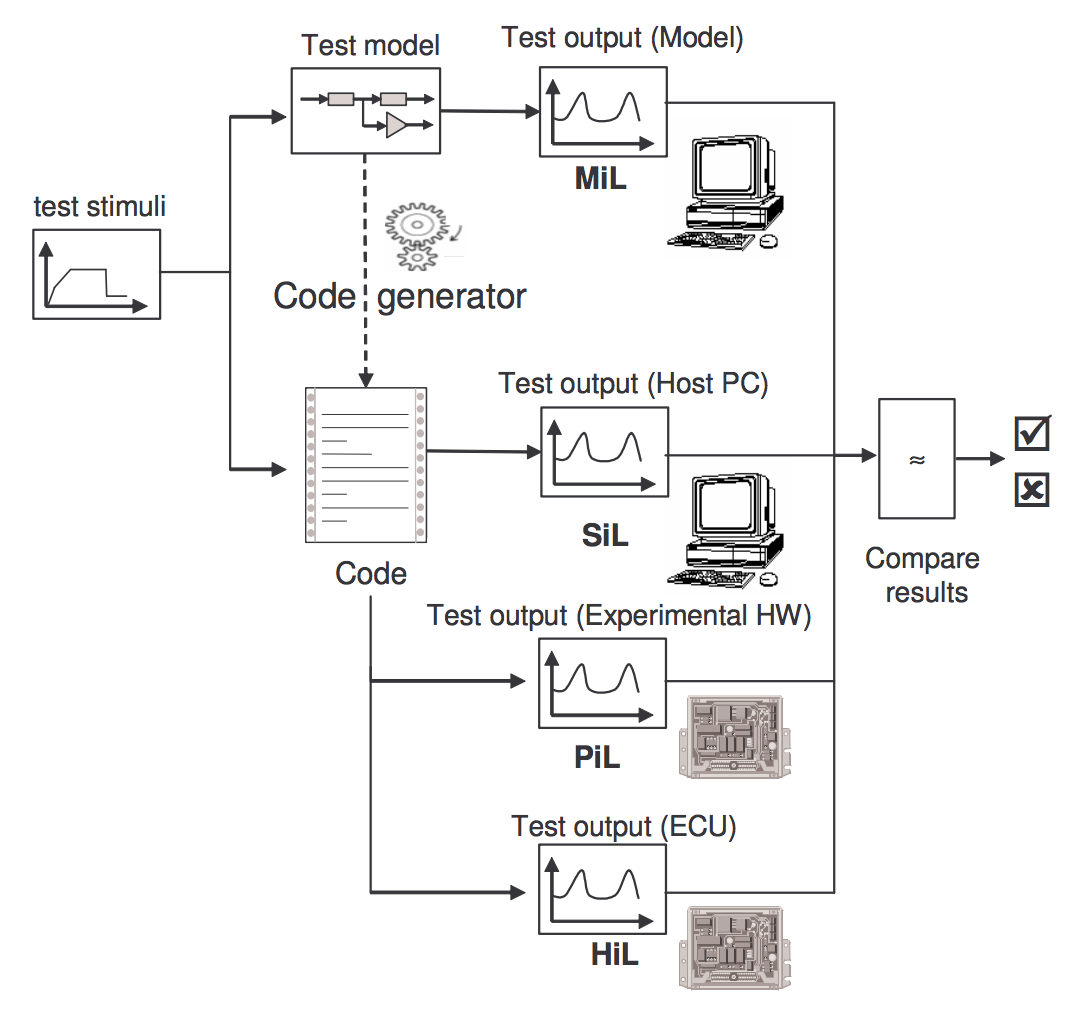
\includegraphics[scale=0.6]{SOTA/fig/testing_process}
	\caption{Automatic functional testing of code generators}
	\label{fig:Process for testing automatically generated code}
\end{figure}

As it is shown in Figure~\ref{fig:Process for testing automatically generated code}, both the generated executable and the simulated model are executed with the same input. 
The determination of the input test stimuli can use a structural testing criteria on model level (model coverage) and code level (code coverage) to generate high-quality test vectors.
Afterwards, the two outputs are compared with respect
to certain acceptance criteria. The comparison procedure is known in the software testing community as equivalence, comparative, or back-to-back testing approach\cite{vouk1990back,mckeeman1998differential}.
 
The great advantage of this approach is that the test oracle is simple to define. It represents the comparison between two or more output results. According to~\cite{shokry2009model,stuermer2007systematic}, there are four stages of comparison that can be performed. They are described as follows (see Figure~\ref{fig:Process for testing automatically generated code}):
 
\begin{itemize}
	\item Model-in-the-Loop (MiL): 
	The simulation of the model on the host machine is termed MiL. 
    The MiL's test purpose is to generate a reference test results (expected values). Moreover, MiL simulation captures the specified behavior of the model that is to be implemented in general-purpose language later on. It also checks the validity of the model with respect to the functional requirements. The only problem that could occur during a MiL execution is that the model would fail to execute.

	\item Software-in-the-Loop (SiL): 
	The execution of the generated object code on the host machine with the same stimuli used for the MiL is termed as SiL. The execution results should be comparable to the results obtained during MiL. 
	The aim of SiL is to detect translation errors such as arithmetical problems, and to measure code coverage.
	Once the system detects a defect, the testing environment should provide the tester with a suitable navigation tool to jump to the erroneous data variable in order to fix it.
	
	\item Processor-in-the-Loop (PiL): 
	PiL tests the object code on the target processor. It generates the cross compiled source code and executes it on the target processor machine. Of course, compiler optimizations can be applied to enhance the code quality. Then, the test scenario is executed on the target processor (\eg, target embedded systems as in~\cite{shokry2009model}). The aim of PiL is to verify the code behavior on the target processor and to measure code efficiency (\eg, profiling, memory usage, etc.).
	
	\item Hardware-in-the-Loop (HiL): 
	Finally, during HiL, the software embedded into the target chip is executed. For that purpose, the target hardware is connected to a real-time simulation system simulating the plant. The model originally developed no longer simulates the physical environment signals, a dedicated hardware is specially designed for this purpose. The aim of HiL is to check the correct software behavior on real hardware.
\end{itemize}

In this context, Conrad \etal\cite{conrad2010code} applied the approach described above by presenting an automated testing approach to assess the equivalence between Simulink models and the generated code. This approach is called Code Generation Verification (CGV).
CGV assesses the numerical equivalence between the model used (\ie, Simulink models) and the generated code (\ie, the executables derived from the generated C Code). 
In fact, each individual model-to-code translation is followed by a verification phase to assess that the input Simulink model used for code generation and the output (\ie, the object code derived from the model via code generation and compilation) produce the same numerical results when stimulated with identical inputs. 
In their equivalence testing approach, they use to run the model used for code generation using simulation and the generated code with the same input stimuli (test vectors) followed by a numerical comparison of the outputs (result vectors).
Then, they check whether or not the semantics of the model have been preserved during code generation, compilation, and linking, by comparing the result vectors, which are the outputs resulting from stimulation with identical test vectors of the model and the generated code.
More precisely, the simulation results should be similar to the execution results. However, when defining the result vector comparison, they tolerate limited differences between both results. They argue that some factors between simulation and execution may cause a small difference between both executions such as limited precision of floating point numbers, target optimized code constructs, etc. 
Thus, they define an application-dependent threshold. So, two result vectors are considered sufficiently similar when their difference is less than a specific threshold value.
They illustrate the CGV-based translation validation in the context of embedded automative software by using Simulink and Real-Time Workshop Embedded Coder for verification. They assess their approach by verifying the numerical equivalence between Simulink models and C generated code. They calculate the absolute difference between simulation results and execution results. Then, they compare this difference to the defined tolerance threshold. They show that for some input test suites there exist mismatched signals (with high variation value) which represent an inconsistency between designed models and executed signal.

In~\cite{conrad2009testing}, the automatic code generation tool is certified to a particular safety standard (IEC 61508-3). Compliance of the model with a standard helps to demonstrate that the model is well-formed according to the certification and that it meets all requirements for later code generation. The process of code generator evaluation (described above) is used to show that the generated code is equivalent to the model (that respect the IEC 61508-3 safety standard)

Stuermer \etal~\cite{stuermer2007systematic} present a systematic test approach for model-based code generators. They investigate the impact of optimization rules for model-based code generation by comparing the output of code and model executions.
If these outputs are equivalent, it is assumed that the code generator works as expected. 
They evaluate the effectiveness of this approach by means of testing optimizations performed by the TargetLink code generator. Test vectors are generated using a structural coverage of the model and generated code.
They have used Simulink as a simulation environment of models. 

In \cite{jorges2014back}, authors present a testing approach of the Genesys code generator framework which tests the translation performed by a code generator from a semantic perspective rather than just checking for syntactic correctness of the generation result. Basically,
Genesys realizes back-to-back testing by executing both the source model as well as the generated code on top of different target platforms. Both executions produce traces and execution footprints are then compared with each other.

Another alternative for validating a code generator would be to use formal proofs\cite{basir2008constructing}. This involves mathematically proving that the code generation transformation process is correct and that each code generation rule preserves the model's semantic. 
Denney \etal\cite{denney2005certifiable} extend an existing code generator such that it produces all logical annotations that are required for formal safety proofs. These proofs certify that the program does not violate certain conditions during its execution. This approach is integrated into the AUTOBAYES and
AUTOFILTER code generators. They used it to prove that the generated code satisfies both language-specific properties such as array-bounds safety or proper variable initialization and domain-specific properties such as vector normalization, matrix symmetry, or correct sensor input usage.

\subsubsection{Summary of functional testing approaches}
Inspired by the work of Sturmer \etal\cite{sturmer2005overview}, we provide a summary of the existing techniques that are applied to test the automatic code generation, some of them are described above: 
	\begin{table}[H]
		\centering
		\caption{Summary of several approaches applied for testing code generators\cite{sturmer2005overview}}
		\noindent\resizebox{\linewidth}{!}{%
		\begin{tabular}{| p{0.12\textwidth} | p{0.25\textwidth} |p{0.6\textwidth} |}\hline
			Level & Testing technique & Objectives \\	\hhline{|=|=|=|}	
			Model 
			& Functional MiL simulation/testing & 
			--Verify that the model reflects its functional requirement specification \\ 
			&& --Check validity of the model within the development environment
			without resource limitations of target environment \\
			\cline{2-3}
			& Structural MiL testing (model coverage) & --Explore possible pathways within the model by determining test cases on the basis of the model structure \\
			\cline{2-3}
			& Adoption of modeling guidelines & --Rely on experiences and expert knowledge\\
			&& --Reveal design errors at an early development stage \\
			\hline
			Code \newline generator  
			& Tool certification & --Independent approval which guarantees that techniques, applied for developing and verifying the tool, are in compliance with the requirements of a certification standard \\
			\cline{2-3}
			& Testing & --Ensure that the code generator has been tested rigorously \\
			&& --Validate that specific translation functions (\eg, optimisations) behave
			as expected \\
			\cline{2-3}
			& Formal proof & --Show by means of mathematical proofs that each code generation (rule) preserves the model’s semantics \\
			\cline{2-3}
			& Adoption of standards and guidelines & --Ensure that the code generator has been developed following a systematic
			development process / quality management system \\ \hline
			Generated code 
			& Functional SiL testing & --Detect translation errors \\
			\cline{2-3}
			& Functional PiL testing & --Check validity of the code behavior taking into account the target CPU architecture \\
			\cline{2-3}
			& Functional HiL testing & --Check behavior of the code when it is deployed in the target harware device \\
			\cline{2-3}
			& Structural MiL/HiL/PiL testing & --Determine test cases on the basis of the code structure and explore possible execution pathways \\
			\cline{2-3}
			& Static analysis & --Check that code conforms to coding guidelines/standards\\
			&& --Detect optimization opportunities such as dead code, etc. \\
			\hline
		\end{tabular}}
		\label{tab:targetlink}
	\end{table}
 
%\cite{sturmer2003test} // talk about ASE paper


\subsection{Non-functional testing of code generators}
\label{sec:Non-functional testing of code generators}
Previous work on non-functional testing of code generators focuses on comparing, as oracle, the non-functional properties of hand-written code to automatically generated code~\cite{stepasyuk2015evaluating,richard2013efficient}. As an example, Strekelj \etal~\cite{vstrekelj2015performance} implemented a simple 2D game in both, the Haxe programming language (a high-level language) and the target programming language, and evaluated the difference in performance between the two versions of code. They showed that the generated code through Haxe has better performance than the hand-written one. 

In \cite{ajwad2007evaluation}, authors compare some non-functional properties of two code generators, the TargetLink code generator and the Real-Time Workshop Embedded Coder. They also compare theses properties to manually written code. The code run on a C166 microprocessor as a target which is an embedded system.
The metrics used for comparison are ROM and RAM memory usage, execution speed, readability, and traceability. Many test cases are executed to see if the controller behaves as expected.
The comparison results show that the generated code by TargetLink is more efficient than the manually-written code and the other generated code in terms of memory and execution time. They also show that the generated code can be easily traced and edited.

Cross-platform mobile development has been also part of the non-functional testing goals since many code generators are increasingly used in industry for automatic cross-platform development. In~\cite{pazirandeh2015evaluation,hartmann2011cross}, authors compared the performance of a set of cross-platform code generators and presented the most efficient tools.



\subsubsection{The oracle problem}
\label{sec:The oracle problem}

%Most of the work on software testing seeks to automate as much as possible the testing process to make it faster, cheaper, and more reliable. Automating this process involves many aspects such as test data generation, test cases generation and execution, test suites reduction, test cases prioritization, etc. Many techniques, especially search-based testing techniques, have been proposed to solve and automate these processes\cite{ali2010systematic}.
%For instance, the problem of automatically generating test inputs/data has been the subject of research interest for a long time. It consists in automatically generating test data/cases in order to detect faults/crashes or to maximize the code coverage of the program under test. 

One of the most important aspects we are interesting in while testing code generators is the \textit{test oracle}. It is the mechanism that verifies whether the outputs of the program for the executed test cases are correct or not.

Compared to many aspects of test automation, the problem of automating the test oracle is still challenging and less well solved. Only few techniques are available to generate test oracles. In most of the cases, designing and implementing test oracles are still manual and expensive activities. That is because the test oracles are not always available and may be hard to define or too difficult to apply\cite{barr2015oracle}. This is commonly known as the \textit{``oracle problem''}. 
As pointed out in\cite{manolache2001software}, the oracle problem has been \textit{``one of the most difficult tasks in software testing''} but it is often ignored by researchers.

In this context, the automatic testing of code generators particularly implies the oracle problem. When testing compilers, for example, it is quite difficult to automatically verify the equivalence between the source code and object code. This task becomes even more complicated when some optimizations are applied to the machine code. 
When testing code generators, the verification of the equivalence between the high-level system specification and the generated code is also challenging.  

As we discussed in Section~\ref{sec: Functional testing of code generators} about the automatic functional testing of code generators, the test oracle is often defined as a back-to-back comparison between the output of the system specification and the generated code.
When it comes to test the non-functional properties such as the resource usage or execution speed, this problem becomes more critical. There is no clear definition about how the oracle should be defined except the few research efforts, discussed in Section~\ref{sec:Non-functional testing of code generators}. 


%SINE + MEtamorphic testing
%When testing a program p supposedly implementing the sine function, for example, let 1.28 be a test case. Although we do not know the exact value of sin1.28, a failure can still be identified if the output p(1.28) > 1 because |sinx| ≤ 1 ∀x ∈ R. By employing more mathematical properties of the sine curve, the range of plausible values of p(1.28) can be further narrowed down greatly.



The research community has proposed several approaches\cite{harman2013comprehensive,barr2015oracle} to alleviate the oracle problem. 
In a recent survey, Harman \etal\cite{harman2013comprehensive} classify test oracles in three categories \textit{specified oracles}, \textit{implicit oracles}, and \textit{derived oracles}. We give an overview of these three categories as they have described:
\begin{itemize}
	\item Specified oracles:
	
	Specified oracles can be generated from several kinds of specifications, such as algebraic specifications or formal models of the system behavior. 
	For example, Stocks \etal\cite{stocks1996framework,richardson1992specification} discuss an approach for deriving test cases and oracles from specification. The idea is that the formal specification of a software can be used as a guide for designing functional tests. Then, test oracles can be associated with individual test templates (test case specifications). Thus, they construct abstract models of expected outputs, called oracle templates. 
	The approach is illustrated with test oracle templates for the \textit{Z} specification.
	
	Specified oracles are effective in identifying errors. However, the task of defining and maintaining specifications is very expensive and time consuming. The applicability of specified oracles is therefore limited and they are also less adopted in industry.
	
	\item Implicit oracles:
	
	Implicit oracle refers to the detection of ‘obvious’ faults such as a program crash, abnormal termination, or execution failure.
	Thus, oracle definition does not require any domain knowledge or formal specification to implement, and as a consequence, it does not need any prerequisites about the behavior or semantics of the program under test.
	
	Implicit oracles\cite{harman2013comprehensive,barr2015oracle} are easy to obtain at practically no cost. At the same time, implicit oracles are mostly incomplete, since they are not able to identify internal problems and complex failures, but they help to detect, in a black-box way, general errors like system crashes or un-handled exceptions.
	
	As an example, fuzz testing\cite{miller1990empirical} is one of the methods where implicit oracles are used to find anomalies, such as crashes. The idea of fuzzing is to generate random inputs and pass them to the system under test to find anomalies.
	Bugs detection is based on the efficiency of generated inputs/data. If an anomaly is detected, the tester reports it by identifying the input triggering it. 
	Fuzzing is commonly used to detect security vulnerabilities, such as buffer overflows, memory leaks, exceptions, etc.\cite{bekrar2011finding}.
	
	Kropp \etal\cite{kropp1998automated} present an approach to test the robustness of the system under test using implicit oracles.
	This approach relies on the creation and execution of invalid input robustness tests. Specifically, these tests are designed to detect crashes and hangs caused by invalid inputs to function calls. The results show that between 42\% and 63\% of components on the POSIX systems measured had robustness problems. 
	
	Ricca and Tonella\cite{ricca2006detecting} focus on developing patterns to detect anomalies. They consider a subset of possible anomalies that can be found in web applications such as navigation problems, hyperlink inconsistencies, etc. Their empirical results show that 60\% of the web applications considered in their study exhibit anomalies and execution failures.
	
	
	\item Derived oracles:
	
	Derived oracles are derived from various artifacts (\eg, documentation, system executions) or properties other than specifications.
	
	For example, in regression testing, oracles can be derived from the executions of previous versions of the software under test. In this case, the derived oracles will verify if the new software version behaves as the original one\cite{mariani2007compatibility}. For example, EvoSuite and Randoop derive test oracles from previous versions of the system under test.
	
	Oracles can also be automatically derived from program invariants\cite{ernst2000quickly}. Invariants can help programmers characterizing aspects of program execution and identifying program properties that must be preserved when modifying code. They report properties that were true over the observed executions of all programs such as \textit{``y = 2*x+3''}, \textit{``array a is sorted''}, etc. The Daikon invariant detector\footnote{https://plse.cs.washington.edu/daikon/} is an open source tool that applies machine learning techniques to infer these invariant properties.
	
	Another type of derived oracles are pseudo-oracles (also known as differential testing, dual coding, and N-version programming\cite{patrick2016testing}). 
	The concept of a pseudo-oracle is introduced by Davis and Weyuker\cite{davis1981pseudo}.
	A pseudo-oracle is program that is capable of providing the expected outputs and check the correctness of the system by comparing the outputs of multiple independent implementations. 
	It checks the consistency of the results of the different software versions of the systems, when the same functionality is executed. An inconsistency can be detected when one or more versions of the system trigger failures. 
	For example, in compiler testing, different versions of the same program are generated by applying some optimizations. The functionality of the program under test remains the same for all versions. The oracle is defined, in this case, as a comparison between the functional outputs of the different versions\cite{yang2011finding}.
	
	Additionally, oracles can be derived from properties of the system under test. For instance, a metamorphic testing (MT) method has been proposed to alleviate the oracle problem\cite{chen2004case}. MT is an automated testing method that employs expected properties of the target functions to test programs without human implication. 
	MT exploits the relation between the inputs and outputs of special test cases of the system under test to derive metamorphic relations (MRs) defined as test oracles for new test cases. 
	MT recommends that, given one or more test cases (called source or original test cases) and their expected outcomes, one or more follow-up test cases can be constructed to verify the necessary properties (\ie, metamorphic relations) of the system or function to be implemented.
	For a given problem, usually more than one MR can be identified. It is therefore important to select suitable MRs for effective bugs detection.

	MT was recently applied for compiler testing. Le \etal\cite{le2014compiler} present an approach called equivalence modulo inputs (EMI) testing. The idea of this approach is to pass different program versions (with same behavior) to the compiler in order to inspect the output similarity after code compilation and execution. So, given a deterministic program $P$ and a set of input values $I$, the authors propose to create equivalent versions of the program by profiling its execution and pruning un-executed code (by identifying the statements not covered by $I$ and mutating or deleting a subset of the dead statements of $P$).
	Once a program and its equivalent variant are constructed, both are used as input to the compiler under test and then, inconsistencies in their results are checked. Inconsistencies represent, in this case, deviations in the functional behavior.
	This method has detected \num{147} confirmed bugs in two open source C compilers, GCC and LLVM.
	EMI testing is an example of metamorphic testing. In fact, the program variants are in a metamorphic relationship with one another and with $P$, with respect to $I$.
	Another application of the equivalence-based method is presented by Tao \etal\cite{tao2010automatic} to test the semantic-soundness property of compilers. They use three different techniques in generating equivalent source code programs and then test the mutants with the original programs, such as replacing an expression with an equivalent one. Empirical results show that their approach is able to detect real issues in GCC and ICC compilers.
	A metamorphic approach has also been used to test GLSL compilers via opaque value injection\cite{donaldson2016metamorphic}.
	
	Pseudo-oracles and metamorphic oracles have similar concept. Pseudo-oracles need different implementations of the same program specification while in metamorphic testing, follow-up test cases (program variants) must be derived from original program under test through program transformations.
	

	
	
\end{itemize}


\subsubsection{Summary: oracle definition approaches}
\label{sec:cg-Summary: oracle definition approaches}
We provide in Table \ref{tab:Summary of test oracle approaches} a summary of the several oracle definition techniques described above:

	\begin{table}[H]
		\centering
		\caption{Summary of test oracle approaches}
		\noindent\resizebox{\linewidth}{!}{%
		\begin{tabular}{| p{0.2\textwidth} | p{0.3\textwidth} |p{0.45\textwidth} |}\hline
			Oracle & Method & Objectives \\	\hhline{|=|=|=|}	
			Specified oracles 
			& --Assertions and contracts\newline  --Specification-based languages\newline  --Algebraic specification languages  & 
			--Use of notions of specifications as a source of oracle information. \\ 
		
			\hline
			Implicit oracles  
			& --Fuzz testing\newline --Load testing\newline --Robustness checking & --Identify obvious faults such as crashes, memory leaks, un-handled exceptions, abnormal program termination, etc. \\
			
			\hline
			Derived oracles 
			& --Metamorphic testing\newline --N-version programming\newline --Regression testing\newline --Back-to-back testing\newline --Invariant detection & --Oracles are derived from various artifacts (\eg, documentation, system executions) or properties (\eg, metamorphic relations) of the system under test.\newline -- Check the consistency of the results of the different versions of the systems, when the same functionality is executed. \\
			
			\hline
		\end{tabular}}
		\label{tab:Summary of test oracle approaches}
	\end{table}

\section{Compilers auto-tuning techniques}
\label{sec:Compilers auto-tuning techniques}

\subsection{Iterative compilation}
Iterative compilation, \textit{also known as optimization phase selection, adaptive compilation, or feedback directed optimization}\cite{triantafyllis2003compiler}, consists in applying software engineering techniques to produce better and more optimized programs. The key objective of iterative compilation is to find the best optimization sequence that leads to the fastest and highest-quality machine code. 
%Our work is related to iterative compilation research field.

The basic idea of iterative compilation is to explore the compiler optimization space by measuring the impact of optimizations on software performance.
Several research efforts have investigated this optimization problem, such as Search-Based Software Engineering (SBSE) techniques, to guide the search towards relevant optimizations regrading performance, energy consumption, code size, compilation time, etc. Experimental results have been usually compared to standard compiler optimization levels.  

It has been proven that optimizations are highly dependent on the target platform and on the input program which makes the task of searching for the best optimization sequence very complex\cite{triantafyllis2003compiler}.

In the following sections, we describe the classical iterative compilation process and we discuss the relevant techniques and approaches that have been presented to tackle some of the challenges related to compiler optimization we have identified in the previous chapter, namely:
\begin{itemize}
	\item \textbf{The problem of optimization-space exploration:} We present several approaches that have addressed the combinatorial explosion problem of possible compiler optimizations.
	
	\item \textbf{The problem of multi-objective optimization:} We present several techniques that aimed to find trade-offs between multiple non-functional properties.
		
	%\item \textbf{The problem of hardware heterogeneity:} Since the optimizations are highly dependent on the input program and on the target platform, we describe for each discussed approach the execution environment used to run the iterative process as well as the evaluation settings.  
\end{itemize}

%Compared to our proposal, none of the previous work has studied the impact of compiler optimizations on resource usage. In this work, we rather focus on compiler optimizations related to resource consumption, while bearing in mind the performance improvement.

\subsection{Implementation of the iterative compilation process}
\begin{figure}[h]
	\center
	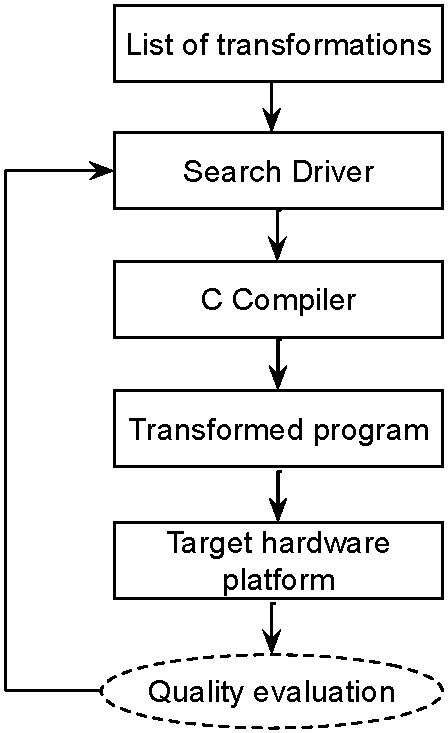
\includegraphics[scale=0.7]{SOTA/fig/iterative_compilation}
	\caption{Overview of the iterative compilation process}
	\label{fig:iterative_compilation}
\end{figure}
The implementation of an iterative compilation system consists mainly on applying a sequence of steps to enhance the quality of the generated code. Figure~\ref{fig:iterative_compilation} shows a general overview of the main steps needed to ensure the implementation of the iterative compilation process.
\begin{itemize}
	\item[--] \textbf{List of transformations:}
	
	The iterative process starts by defining the optimization space. It represents the list of optimizations that the compiler has to evolve during the search for the best optimization sequences.
	
	\item[--] \textbf{Search engine:}
	
	It applies a search algorithm or method to efficiently explore the large optimization search space. In fact, it takes as input the previously defined list of transformations and decides which optimizations will be retained at the end of the search.
	
	\item[--] \textbf{C Compiler:}
	
	Once the optimization sequence is defined, the target C compiler is called to compile the input program and also perform initial machine independent optimizations. 
	
	\item[--] \textbf{Machine-independent optimizations:}
	
	This results in an initial machine independent optimized program. These optimizations are performed during code generation and impact all target systems. It includes optimizations that are applied during the parse tree mapping to the intermediate code and the optimization applied to the intermediate code itself.
	
	\item[--] \textbf{Machine-dependent optimizations:}
	
	For further optimization, the compiler applies from the provided optimization sequence the machine dependent optimizations. This includes optimizations applied during the mapping of intermediate code to assembler and optimizations applied directly on the generated object code.
	
	\item[--] \textbf{Quality evaluation:}
	
	It consists on evaluating the quality of the optimized code. Many non-functional properties can be evaluated like code size, execution time, resource usage, power consumption, etc.
	
\end{itemize}

This model represents the classical and typical iterative compilation process. Of course, there exist many ways and adaptations to implement this process. The implementation of the iterative process depends on the algorithm used, the problem addressed, the technologies used, etc. The goal of the next subsections is to present the different state of the art approaches related to iterative compilation.

\subsection{Iterative compilation search techniques}
In Section~\ref{sec:Why compilers auto-tuning is complex?} of Chapter~\ref{chap:background}, we presented several issues with optimizing compilers that make the activity of compiler auto-tuning very complex such as the huge number of optimizations, conflicting objectives, optimization impact, etc.
In this section, we discuss the available tools and approaches dedicated to the automatic search for optimal compiler settings, and give an overview of known approaches that addressed these several compiler optimization challenges. In each subsection, we identify and discuss a particular problem and we present the best known approaches proposed to solve it.

\subsubsection{Auto-tuning: a mono objective optimization}
The compiler auto-tuning technique has been used in many optimization scenarios.
What all of this prior work on iterative compilation has in common is that it focuses on a single objective function to be optimized. For example, researchers typically focus on speeding up the performance of compiled code which constitutes the major optimization objective for most iterative compilation approaches\cite{pan2006fast,haneda2005automatic,almagor2004finding,fursin2002evaluating,chen2010evaluating,cooper1999optimizing}. 

So, the problem has been often adapted as a mono-objective search problem where the speedup is the main concern for most of the previous work. 
Genetic algorithms (GA)\cite{stephenson2003genetic,bashkansky2007black} present an attractive solution to this problem. 
GA-based approaches compute an initial population using a set of optimizations, generally defined under the standard compiler levels -Ox. Then, at each iteration, the individuals (\ie, option sets) that comprise the generation are evaluated by measuring the execution time of each solution. The results are sorted and pass through a breeding and mutation stage to form the next generation. This
process continues until a termination condition is reached. At the end, the algorithm returns the best optimization set that led to the highest performance.

For example, ACOVEA\footnote{https://github.com/Acovea/libacovea} (Analysis of Compiler Options via Evolutionary Algorithm), is an open source tool that applies GAs to find the best options for compiling programs with the GCC compiler. In this context, best solutions define those options that produce the fastest executable program from a given source code. This tool was even included in the Gentoo Linux repository to help users to find the best set of optimizations.

The ESTO framework\cite{bashkansky2007black} studies the application of GA to the problem of selecting an optimal option set for a specific application and workload. ESTO regards the compiler as a black box, specified by its external-visible optimization options. ESTO supports a GA variant named budget-limited genetic algorithm which reduces the population size exponentially and then reduce the time needed to evaluate the different evaluations. The authors ran experiments on the SPEC2000 benchmark suite and tested 60 optimization options within three compilers: GCC, XLC and FDPR-Pro. Results of ESTO are compared to GCC -O1 and -O3, to XLC -O3, and to FDPR-Pro -O3. The results show that ESTO is capable to construct optimization levels that yield to better performance than standard options.

%\subsubsection{JIT compiler optimization}

%\subsubsection{Dealing with numerical parameter values}
%The phase ordering problem is a common problem in iterative compilation. It is related to numerical parameters optimization where the parameter optimization value should be determined automatically.

\subsubsection{Escaping local optimum}


A common problem in iterative compilation is the local optimum. In fact, the search space of optimizations for a specific program could be very huge and it generally contains many local minima in where the search algorithm could be trapped\cite{bodin1998iterative}. Therefore, researchers in this filed try to build robust techniques and algorithms to avoid such problem.
In~\cite{bodin1998iterative}, Bodin \etal tried to analyze this search space and they found that the optimization space is highly non-linear containing many local minima and some discontinuities.
This paper focuses on parameterized transformations. The small area of the transformation space considered in this paper is composed of three parameterized optimizations: loop unrolling (with unroll factors from 1 to 20), loop tiling (with tile sizes from 1 to 100) and padding (from 1 to 100). They focus on reducing the compilation and execution time of optimized programs and use a simulator to target embedded processors. They use a compiler framework developed to optimize multimedia programs for embedded systems.
They analyze these optimizations across four CPU architectures (UltraSparc, R10000, Pentium Pro, and TriMedia-1000) and the matrix multiplication is selected as the program to optimize.
The proposed search algorithm visits a number of points at spaced intervals, applying the appropriate transformation, executing the transformed program and evaluating its worth by measuring the execution time. Those points lying between the current global minimum and the average are added to an ordered queue. Iteratively, such points are removed from the queue and points within the neighboring region are investigated, again at spaced intervals. This process is continued until a specific number of points are evaluated and the fastest transformed program is reported.
They show that in the case of large transformation spaces, they can achieve within 0.3\% of the best possible time by visiting, less then 0.25\% of the space. They find the minimum after visiting up to less than 1\% of the space.

Cooper \etal\cite{cooper2006exploring} describe their experience exploring the search space of compilation sequences. They report the results of exhaustively enumerating several search spaces of sequences of length 10 chosen from 5 transformations. They show that the search space has many local minima, and that random-restart hill climbing is an effective strategy to overcome this problem.


Another way to efficiently explore the large search space in compiler optimization is the Design Space Exploration (DSE) technique\cite{martins2014exploration,martins2016clustering}. The DSE is based on a clustering approach for grouping functions with similarities and exploration of a reduced search space resulting from the combination of optimizations previously suggested for the functions in each group.
The identification of similarities between functions uses a data mining method that is applied to a symbolic code representation.
They compare their approach to the GA and their experimental results reveal that the DSE-based approach achieves a significant reduction in the total exploration time of the search space (20x over a GA approach) and a performance speedup (41\% over the baseline). 



%paper: Exhaustive Optimization Phase Order Space Exploration
%Earlier work in iterative compilation concentrated on finding good parameter settings for a few optimizations, such as loop unrolling and loop tiling\cite{bodin1998iterative}. In cases where exhaustive exploration was expensive, researchers
%used heuristic algorithms, such as grid-based searches, hill climbers, and genetic algorithms, to scan only a portion of the search space. A common deduction is that typical program search spaces, on a variety of different architectures, generally contain enough local minima that biased sampling techniques should find good solutions.

\subsubsection{Phase ordering problem}
Phase ordering is also an important problem in iterative compilation which explores the effect of different orderings of optimization phases on program performance. In fact, when using some compilers such as LLVM, it is important to define the right order of applying optimizations. Thus, researchers in this field try to apply search techniques in order to find the right optimization sequence. However, reordering optimization phases is extremely hard to support in most production systems, including GCC due to their use of multiple intermediate formats and complex inherent dependencies between optimizations. So generally, compilers manage internally the order of applying optimizations and do not give the hand to the user to choose this order, avoiding conflicts and compilation issues.

When the order is managed by the users, exhaustively evaluating  all orderings of optimization phases is infeasible due to the huge number optimization phases. This problem becomes more complex by the fact that these phases interact with other optimizations in a complex way.
For example, even if we keep the same set of optimizations for an input program, varying the order of applying these optimization phases can produce different code, with potentially significant performance variations amongst them. 

In this field, Whitfield\cite{whitfield1990approach} developed a framework based on axiomatic specifications of optimizations, including both \textit{pre} and \textit{post} conditions before and after applying optimizations. For a selected set of optimizations, the framework is used to determine those interactions among the optimizations that can create conditions and those that can destroy conditions for applying other optimizations. Then, from these interactions, an application order is derived to obtain the potential benefits of the optimizations that can be applied to a program. 
This framework was employed to list the potential enabling and disabling interactions between optimizations, which were then used to derive an application
order for the optimizations

Kulkarni \etal\cite{kulkarni2009practical,kulkarni2006exhaustive} proposed an exhaustive search strategy to find optimal compilation sequences for each function of a program. They exhaustively enumerated all distinct function instances for a set of programs that would be produced from different phase-orderings of 15 optimizations. This exhaustive enumeration was made possible by detecting which phases were active and whether or not the generated code was unique, making the actual optimization phase order space much smaller than the attempted space. This exhaustive enumeration allowed them to construct probabilities of enabling/disabling interactions between different optimization passes in general and not specific to any program. They use this idea to prevent the combinatorial explosion of the total number of sequences to be tested. 
They were able to find all possible function instances that can be produced by different phase orderings for 109 out of the 111 total functions they evaluated.


Cooper \etal\cite{cooper1999optimizing} adapts the GA to solve the optimization phase ordering problem. They target embedded systems and focus on reducing the code size. They choose 10 program transformations to evolve in Fortran compiler. The solutions generated by their algorithm are compared to solutions found using a fixed optimization sequence. Their technique was successful for reducing the code size by 40\% compared to the standard sequence.

In another work\cite{cooper2006exploring}, the same authors explored phase orders at program-level with randomized search algorithms based on GAs, hill climbers, and randomized sampling. They target a simulated abstract RISC-based processor with a research compiler. They report properties of several generated sub-spaces of phase ordering and the consequences of those properties for the search algorithms.

\subsubsection{Evaluating iterative optimization across multiple data sets}
Most iterative optimization studies find the best compiler optimizations through repeated runs on the same data set. The problem is that if we select the best optimization sequence for an input data set through the iterative process, we do not know if it will still be the best for the same program but with other data sets. Thereby, researchers in this field try to investigate this problem by evaluating the effectiveness of iterative optimization across a large number of data sets. In particular, since there is no existing benchmark suite with a large number of data sets, Chen \etal\cite{chen2010evaluating} attempt to collect 1000 data sets called KDataSets for 32 programs, mostly derived from the MiBench benchmark. Then, they exercise iterative optimization on these collected data sets in order to find the best optimization combination across all data sets. 
They use random search to generate random optimization sequences for the ICC compiler (53 flags) and the GCC compiler (132 optimizations).
They demonstrate that for all 32 programs (from MiBench), they were able to find at least one combination of compiler optimizations that achieves 86\% or more of the best possible speedup across all data sets using ICC (83\% for GNU’s GCC). This optimal combination is program-specific and yields speedups up to 1.71 on ICC and 2.23 on GCC over the highest optimization level (-Ofast and -O3, respectively). This means that a program can be optimized on a collection of data sets and it can retain near optimal performance for most other data sets. However, they tested their approach on only one single benchmark and one target architecture.

\subsubsection{Conflicting objectives: a multi-objective optimization}
Several research efforts attempt to find trade-offs between two (or more) non-functional properties~\cite{almagor2004finding,hoste2008cole,pan2006fast,pallister2015identifying,chen2012deconstructing,martins2014exploration,lin2008automatic,martinez2014multi}.

In COLE\cite{hoste2008cole}, the authors considered that the problem of compiler optimizations can be seen as a multi-objective problem where two non-functional properties can be enhanced simultaneously. Thus, they investigated the standard levels of compiler optimization by searching for pareto optimal levels that maximize both performance and compile time. 
They show that by using the multi-objective genetic algorithm (in their experiment they used SPEA2), it is possible to find a set of compiler optimization sequences that are more pareto-effective in terms of performance and compile time than the standard optimization levels (-O1, -O2, -O3, and -Os). The motivation behind this approach is that these standard levels were set up manually by compiler creators based on fixed benchmarks and data sets. For the authors, these universal levels may not be always effective on unseen programs and there exist higher levels that provide better trade-offs in terms of code quality.
They used the SPEC2000 CPU benchmark, which is a popular benchmark suite for evaluating the compiler performance. They evolved 60 optimization flags that are defined in the standard levels -O1, -O2, -O3, and -Os. They run iterative compilation on one single machine shipped with Intel CPU Pentium 4 and they compared the proposed algorithm (SPEA2) to random search as well as to standard optimization levels.
The experimental results using GCC (v4.1.2) show that the automatic construction of optimization levels is feasible in practice, and in addition, yields better optimization levels than GCC’s manually derived optimization levels.
However, they do not provide a guarantee that the new explored optimization levels will be optimal for other applications.


Martinez \etal\cite{martinez2014multi} propose an adaptive worst-case execution time aware compiler framework for automatic search of compiler optimization sequences. 
Compared to the previously described approaches, authors in this work focus on generating efficient code for embedded systems. Therefore, they focus on crucial properties for real-time systems such as average-case execution time (ACET), worst-case execution time (WCET), power consumption and code size. 
They explore the performance of compiler optimizations with conflicting goals. Thus, they try to find suitable trade-offs between these objectives in order to identify pareto optimal solutions using multi-objective algorithms. The objective functions try to minimize the WCET-ACET and WCET-Code size properties. They apply three evolutionary multi-objective algorithms namely IBEA, NSGA-II and SPEA2 and compare their results to standard levels (-O1, -O2 and -O3). 
They evolve 30 optimizations within the WCC compiler and perform experiments on top of one single machine shipped with Intel Quad-Core CPU processor. They pick up 35  programs from various benchmarks such as DSPstone, MediaBench, MiBench, etc.
They find that NSGA-II is the most promising algorithm for the given problem. The discovered optimization sequences significantly outperform standard optimization levels. In fact, the highest standard optimization level -O3 can be outperformed for the WCET and ACET on average by up to 31.33\% and 27.43\%, respectively. The same approach performs as well for the WCET-Code size optimization with a 30.6\% WCET reduction over -O3. However, the code size increases by 133.4\%. They argue that the WCET and the code size are typical conflicting goals. If a high improvement of one objective function is desired, a significant degradation of the other objective must be accepted.

In~\cite{plotnikov2013automatic}, the TACT framework is presented. 
Compared to previous approaches, TACT is designed primarily for automatic tuning on embedded systems running Linux. Thus, the target CPU architecture for this tool is the ARM architecture (ARM Cortex-A9) and 200 options are used in the GCC compiler for ARM. 
TACT supports multiple optimization objectives, so it can tune either for a single optimization parameter, or for two objective functions simultaneously, for example, for performance and code size (or compile time). So, it applies the SPEA2 algorithm and GA for mono-objective optimizations.
The results show how the SPEA2 outperforms the standard GCC levels (-O2, -O3 and -Os) across several open-source popular applications such as  C-Ray, Crafty Chess, SciMark, x264 and zlib.


 

\subsubsection{Predicting optimizations: a machine learning optimization}
Machine learning has been also proposed by several research efforts to tune compilers. Compared to evolutionary algorithms, using machine learning in compiler optimization has the potential of reusing knowledge across the different iterative compilation runs, gaining the benefits of iterative compilation to learn the best optimizations across multiple programs and architectures.

Generally, machine learning application create in an offline phase a prediction model, which will be used to determine the compiler optimization set that should be applied to unseen programs in the online phase. The main advantage of this technique is to reduce the number of required program evaluations.

In the Milepost project\cite{fursin2011milepost} for example, authors start from the observation that similar programs may exhibit similar behavior and require similar optimizations, so it is possible to correlate program features and optimizations together to predict good transformations for unseen programs, based on previous optimization experience. Thereby, they provide a modular, extensible, self-tuning optimization infrastructure that can automatically learn how to best optimize programs for configurable heterogeneous processors based on the correlation between program features, run-time behavior and optimizations. 
The proposed infrastructure is based on a machine learning compiler that presents an Interactive Compilation Interface (ICI) and plugins to extract program features (such as the number of instructions in a method, number of branches, etc) and select optimization passes. 

The Milepost framework proceeds in two distinct phases: training and deployment. During the training phase, information about the structure of programs (input training programs) is gathered, showing how they behave under different optimization settings. Such information allows machine learning tools to correlate aspects of program structure, or features, with optimizations, building a strategy that predicts good combinations of optimizations. 
After running an iterative process that evaluates different combinations of optimizations on top of the training programs/features, predictive models are created to correlate a given set of program features with profitable program transformations. 
Then, in the deployment phase, the framework analyzes new unseen programs by determining the program features and passes them to the new created models to predict the most profitable optimizations to improve execution time or other metrics depending on the user’s optimization requirements.
GCC was selected as the compiler infrastructure. They evolved 100 optimization flags under -O1, -O2 and -O3 levels and compared their results to the -O3 level and to the random search.
The experimental results show that it is possible to improve the performance of the MiBench benchmark suite automatically using iterative compilation and machine learning on several platforms, including x86: Intel and AMD, and the ARC configurable core family. Using the machine learning-based framework, they were also able to learn a model that automatically improves the execution time of some individual MiBench programs by a factor of more than 2 while improving the overall MiBench suite by 11\% on reconfigurable ARC architecture, without sacrificing code size or compilation time. Furthermore, their approach supports general multi-objective optimization where a user can choose to minimize not only the execution time but also the code size and compilation time.



\subsubsection{Summary: auto-tuning compiler techniques}
We provide in Table~\ref{tab:Summary of iterative compilation} a summary of several iterative compilation approaches, most of them are described above. We classify these approaches based on the problem they are tackling. Sometimes, the research papers address more than one issue in iterative compilation. This is not an exhaustive study of all iterative approaches but, it gives an overview of several research efforts involved in different areas during the past 20 years.

\begin{table}[H]
	\centering
	\caption{Summary of iterative compilation approaches}
	\noindent\resizebox{\linewidth}{!}{%
	\begin{tabular}{|c|c|c|c|c|c|c|c|}\hline
		   & \shortstack{Local\\ optimum} & \shortstack{Phase\\ ordering} & \shortstack{Multiple\\ data sets} & \shortstack{Conflicting\\ objectives} & \shortstack{Learning\\ Methods} & \shortstack{Multiple\\ CPUs} & \shortstack{Multiple-\\ compilers}\\ \hhline{|=|=|=|=|=|=|=|=|}	
\shortstack{Whitfield \etal'90\\\cite{whitfield1990approach}} & - & + & - & - & - & - & -\\\hline		 
\shortstack{Bodin \etal'98\\\cite{bodin1998iterative}} & + & - & - & - & - & + & - \\\hline
\shortstack{Kulkarni \etal'06\\\cite{kulkarni2006exhaustive}} & - & + & - & - & - & - & - \\\hline
\shortstack{Cooper \etal'06\\\cite{cooper2006exploring}} & + & + & - & - & - & + & - \\\hline
\shortstack{Bashkansky \etal'07\\\cite{bashkansky2007black}} & - & - & - & - & - & + & + \\\hline 
\shortstack{Hoste \etal'08\\\cite{hoste2008cole}} & - & - & - & + & - & - & - \\\hline
\shortstack{Lokuciejewski \etal'10\\\cite{lokuciejewski2010multi}} & - & - & - & + & - & - & - \\\hline
\shortstack{Chen \etal'10\\\cite{chen2010evaluating}} & - & - & + & - & - & + & + \\\hline 
\shortstack{Fursin \etal'11\\\cite{fursin2011milepost}} & - & - & - & + & + & + & - \\\hline
\shortstack{Pekhimenko \etal'11\\\cite{pekhimenko2011efficient}} & - & - & - & + & + & - & - \\\hline
\shortstack{Plotnikov \etal'13\\\cite{plotnikov2013automatic}} & - & - & - & + & - & - & - \\\hline


	\end{tabular}}
	\label{tab:Summary of iterative compilation}
\end{table}



\section{Lightweight system virtualization for automatic software testing}
\label{sec:Lightweight system virtualization for software testing}

The key objective of this section is to present examples of the existing research efforts that have been presented to address:
\begin{itemize}
	\item \textbf{The problem of hardware heterogeneity and software diversity:} For instance, we show the benefit of using a container-based infrastructure to tackle this problem. Thus, we present several research efforts that opted for this technology to facilitate software testing. 
	
	\item \textbf{The problem of resource usage monitoring:} We discuss existing solutions applied for automatic resource usage extraction in a micro-services infrastructure. 
\end{itemize}


Using virtual machines (VMs) as a mechanism for deploying and testing applications in heterogeneous environment is very useful.
In industry, a number of commercial usage scenarios benefit from virtualization techniques to provide services to the end users. For example, Amazon EC2 makes VMs available to the customers who can use them to run their own computer applications or services on the cloud. Thus, a user can create, launch and terminate new VMs as needed.  
However, VMs are known to be very expensive in terms of system resources and performance. In fact, each new VM instance constitutes of a virtual copy of all the hardware of the host machine which increases resource usage and overhead\cite{merkel2014docker}. 
Container-based virtualization presents an interesting alternative technology to VMs. The container technology is an operating-system-level virtualization which imposes little to near zero overhead. Programs in virtual instances use the operating system's system call interface and do not need to be emulated or ran in an intermediate virtual machine, as it is the case for VMware, QEMU or Xen.
For instance, Docker\footnote{\url{https://www.docker.com}} is a popular engine that offers the ability to deploy applications and their dependencies into lightweight containers that are very cheap to create. Processes executing in a Docker container are isolated from processes running on the host OS or in other Docker containers. The Docker solution aims to address the challenges of resource usage and performance overhead caused by the full-stack virtualization. 

Several authors~\cite{spoiala2016performance,soltesz2007container,merkel2014docker,felter2015updated} compared the performance of the traditional VM solution to the container-based operating system technology. They showed that containers result in better performance than VMs since they induce less overhead. 


\subsection{Application in software testing}  
In software development, the container technology becomes more and more used in order to create a portable, consistent operating environment for development, deployment, and testing in the cloud~\cite{li2015rest}.
In the following, we discuss some of the state of the art approaches that choose the container technology as an efficient infrastructure to solve some testing research problems. 

Marinescu \etal\cite{marinescu2014covrig} have used Docker as technological basis in their repository analysis framework Covrig to conduct a large-scale and yet safe inspection of the revision history from six selected Git code repositories. 
For their analysis, they run each version of a system in isolation and collect static and dynamic software metrics, using a lightweight container environment that can be deployed on a cluster of local or cloud machines. Each container is used to configure, compile, and test one program revision, as well as collect the metrics of interest, such as code size and coverage.
The motivation of using such infrastructure is to provide a clean and configurable execution environment to run experiments. According to the authors, the use of Docker as a solution to automatically deploy and execute the different program reversions has clearly facilitated the testing process.


Another Docker-based approach is presented in the BenchFlow2 project which focuses on benchmarking BPMN 2.0 engines\cite{ferme2015framework}. This project is dedicated to the performance testing of workflow engines. In this work, Ferme \etal present a framework for automatic and reliable calculation of performance metrics for BPMN 2.0 Workflow Management Systems (WfMSs). 
According to the authors, benchmarking WfMSs raises many challenges: 1) the system deployment complexity due to the distributed nature of these models execution; 2) the high number of configuration options required to integrate the deployment of the system under test, \ie, the WfMS; 3) the complexity of the execution behaviors that can be expressed by modern modeling and execution languages such as BPMN2.
Therefore, to address these problems, BenchFlow exploits Docker as a containerization technology, to enable the automatic deployment and configuration of the WfMSs.
Thus, the WfMSs are automatically deployed and undeployed using Docker. Each component involved in the benchmark are packaged as Docker images
to be deployed and executed on different servers connected by a dedicated local
network. For each Docker instance, a new instance of the business models set is executed by the Wf during the experiment.
Thanks to Docker, BenchFlow automatically collects all the data needed to compute the performance metrics, and to check the correct execution of the tests (metrics related the RAM/CPU usage and execution time).
Their experimental results show that a simple business model running on two popular
open-source WfMSs reveal important performance scalability issues. 

Hamdy \etal\cite{hamdy2016web} propose Pons, a web based tool for the distribution of pre-release mobile
applications for the purpose of manual testing. Pons facilitates building, running, and manually testing of Android applications directly in the browser. 
Based on Docker technology, this tool gets the developers and end users engaged in testing the applications in one
place, alleviating the tester's burden of installing and maintaining testing environments, and providing a platform for developers to rapidly iterate on the software and integrate changes over time. Thus, it speeds up the testing process and reduces its cost.
Pons utilizes Docker by predefining Docker images that
contain the required services and tools to build Android applications, starting from the operating system up to the
software development kit. A container is then built using one of these images to store the source code of
a mobile application at a specific moment of history in a
sandbox environment. Pons creates then, an Android emulator inside the Docker container to run the tests. The results are streamed at runtime in the web browser.

\subsection{Application in runtime monitoring} 
Runtime monitoring is important in the area of cloud computing\cite{aceto2013cloud}. Like VMs before them, containers require a monitoring mechanism. It should provide both historical and timely information about the resource usage of containers.

In industry, many commercial solutions are proposed to efficiently monitor applications running inside containers. For example, the Datadog\footnote{\url{www.datadoghq.com}} and cAdvisor\footnote{\url{https://github.com/google/cadvisor}} agents use the native Docker accounting metrics to gather the CPU, memory, network, and I/O metrics of the running containers. CAdvisor allows to monitor containers that run in the same host machine. As an alternative, Scout\footnote{https://scoutapp.com} is used to aggregate metrics from different hosts and containers in a distributed architecture.
As an orchestration system for Docker containers, we cite the open project Kubernetes\footnote{https://kubernetes.io}. It allows to quickly and efficiently respond to customer demand by deploying applications using multiple hosts and containers on the cloud. This clustering framework is shipped with a monitoring tool called Heapster\footnote{https://github.com/kubernetes/heapster} that provides a base monitoring platform on Kubernetes. Heapster collects and interprets various signals like resource usage, lifecycle events, etc, and exports cluster metrics via REST endpoints. It supports a pluggable storage backend such as InfluxDB with Grafana and Google Cloud Monitoring.
Most of these tools provide web-based dashboards to visualize resource consumption at runtime as well as alerting mechanism that can be triggered if metrics go above or below a configured threshold. Other examples of Docker monitoring tools exist such as: Sensu Monitoring Framework, Prometheus, Sysdig Cloud, etc.

The runtime monitoring of containers has been also applied to solve research problems. For instance, Kookarinrat \etal\cite{kookarinrat2015analysis} have investigated the problem of auto-sharding in NoSQL databases using a container-based infrastructure for runtime monitoring. 
The auto-sharding technique is used to divide data in the database and distribute it over multiple machines in order to scale it horizontally. In fact, selecting the right key is challenging. It could lead to either an improvement of the performance and capability of a database or to performance issues (\ie, by selecting a wrong key) which could lead to a system halt. 
Therefore, authors analyzed and evaluated such suggested properties by studying how the variation of a shard key’s choices could impact the DB performance.
They simulated an environment using Docker containers and measured the read/write performance of variety of keys. Inside each container, they executed write/read queries into the MongoDB database and used Docker stats to retrieve automatically information about the memory and CPU usage.


Sun \etal~\cite{sun2016roar} present a tool to test, optimize, and automate cloud resource allocation decisions to meet QoS goals for web applications. Their infrastructure relies on Docker to gather information about the resource usage of deployed web servers. 

Containers monitoring has been applied in other research efforts related especially to cloud computing and virtualization\cite{peinl2016docker,medel2016modelling}.
\section{Summary \& open challenges}
\label{sec:suumary SOTA}

The analysis of the state of the art reveals several challenges. We describe below some of the challenges we have identified in both areas of iterative compilation and code generator testing:
%In reviewing the state of the art of resource management for software abstractions, we realized that severe shortcomings in existing approaches prevent their usage in production environments. With regard to the matter of dealing with abstraction-specific features, the following issues exist:
\begin{itemize}
	
\item \textbf{Limits of existing work when testing code generators (the oracle problem):} Most of the work related to the automatic testing of code generators define an equivalence functional oracle to compare the result of MiL, SiL and PiL. In case of non-executable models, this comparison becomes impossible. Particularly, the oracle problem for testing the non-functional properties of the generated code  has been avoided and not addressed by existing research efforts. The only comparison that has been made consists in comparing the hand-written code to the automatically generated code. The key objective of this comparison is to show that the generated code has better or equivalent performance properties compared to the human code.\newline
\textbf{$\Rightarrow$ 
	We believe that more advanced testing techniques as described in Section~\ref{sec:The oracle problem} can be applied to automatically detect code generator issues.}
	
\item \textbf{Limits of existing techniques when exploring the large optimization search space (a multimodal problem):}
As showed earlier, different techniques are applied during the iterative compilation process to explore the large optimization search space. It has been showed that the optimization search space is a multimodal problem, containing many local optima.
For effective search, some authors use to involve only few optimizations (2 to 10) or to prune some paths in order to reduce this large search space.
Genetic Algorithms are largely applied in most of the previous works. However, this technique may fall in the local optimum problem. 
\newline
\textbf{$\Rightarrow$ The optimization search space is multimodal and very large. An alternative solution to the classical approaches is needed to tackle this problem.}
%\item \textbf{Benchmark evaluation:}
	
\item \textbf{Lack of solutions that deal with conflicting objectives when auto-tuning compilers (a multi-objective optimization problem):} 
When trying to optimize software performance, many non-functional properties and design constraints
must be involved and satisfied simultaneously to better optimize code. However, improving program
execution time can result in a high resource usage which may decrease system performance especially for resource-constrained devices. Therefore, it is important to construct optimization levels that represent multiple trade-offs between resource usage and performance, enabling the user to choose among different optimal solutions which best suit the system requirements. Actually, there are only few work that address the compiler optimization as a multi-objective optimization problem. 
\newline
\textbf{$\Rightarrow$ To deal with conflicting objectives, it is important to find a consensus between several non-functional properties when optimizing code to handle both, the resource usage and performance requirements}


\item \textbf{Limits of existing approaches to handle the software platform and hardware requirements (the problem of software diversity and hardware heterogeneity):} Testing generators requires the execution of the generated code on different hardware and software platforms. Most of the existing research techniques apply a naive approach by running the generated code on different machines or using simulators for some configurations. Configuring the target execution environment to run the generated code and test it is time-consuming. Particularly, for generator users, it becomes very difficult to deploy and test the generated software artifacts in front of the increasing diversity of hardware and software platform settings.\newline
\textbf{$\Rightarrow$ A highly configurable execution environment is needed to handle the software and hardware requirements.} 

\item \textbf{Lack of solutions that evaluate the resource usage properties when evaluating the generated code:} There is almost no research effort to deal with the non-functional properties of automatically generated code such as the resource usage. Most of the related work (in code generator testing) focus on the functional correctness of the generated code without putting too much emphasizes on the quality of the generated code. We claim that evaluating properties such as resource usage is very important in order to ensure an efficient production code generation. In iterative compilation, most of the existing work tend to reduce the execution time, code size, compilation time, etc. There is almost no work that evaluates the memory and CPU usage of the optimized code.
\newline
\textbf{$\Rightarrow$ An effective monitoring solution is needed to evaluate the resource usage properties of automatically generated code}
  
\end{itemize}
\iffalse
Our work is related to iterative compilation research field.
The basic idea of iterative compilation is to explore the compiler optimization space by measuring the impact of optimizations on software performance.
Several research efforts have investigated this optimization problem to catch relevant optimizations regrading performance, energy or code size improvements over standard optimization sequences~\cite{almagor2004finding,hoste2008cole,pan2006fast,zhong2009tuning,pallister2015identifying,chen2012deconstructing,sandran2012genetic,martins2014exploration,fursin2008milepost,lin2008automatic,schulte2014post}. 
The vast majority of the work on iterative compilation focuses on increasing the speedup of new optimized code compared to standard optimizations. 
It has been proven that optimizations are highly dependent on target platform and input program. Compared to our proposal, we rather focus on comparing the resource consumption of optimized code.

Novelty Search has never been applied in the filed of iterative compilation. Our work presents the first attempt to introduce diversity in optimization sequences generation. The idea of NS has been introduced by Lehman \etal~\cite{lehman2008exploiting}. It has been often evaluated in deceptive tasks and especially applied to evolutionary robotics~\cite{risi2010evolving,krvcah2012solving} (in the context of neuroevolution). 
NS can easily be adapted to different research fields. In a previous work~\cite{boussaa2015novelty}, NS has been adapted for test data generation where novelty score was calculated as the Manhattan distance between the different vectors representing test data.
In our NS adaptation, we are measuring the novelty score using the systematic difference between optimization sequences of GCC.

For code generators testing, Stuermer \etal present a systematic test approach for model-based code generators~\cite{stuermer2007systematic}. They investigate the impact of optimization rules for model-based code generation by comparing the output of the code execution with the output of the model execution. 
If these outputs are equivalent, it is assumed that the code generator works as expected. 
They evaluate the effectiveness of this approach by means of testing optimizations performed by the TargetLink code generator. 
They have used Simulink as a simulation environment of models. 
In our approach, we provide a component-based infrastructure to compare non-functional properties of generated code rather than functional ones. 
\fi
